\hypertarget{en-route-sur-la-great-ocean-road}{%
\section{En route sur la Great Ocean
Road}\label{en-route-sur-la-great-ocean-road}}

\emph{Mardi 31 juillet 2018}

Même si cela ne faisait pas partie de nos plans initiaux (qui étaient en
fait inexistants, avouons-le), nous avons passé les derniers jours à
parcourir un bout d'Australie en voiture. Et cela a été une très belle
expérience (au prix d'encore plus de CO2 sous forme de billets d'avion).

Alors, c'est quoi cette Great Ocean Road ? C'est une route
\emph{scénique} d'environ 300 kilomètres qui, comme son nom le suggère,
serpente le long de l'océan entre Geelong, près de Melbourne, jusqu'à
Warrnambool, vers l'ouest. Construite par des hommes qui avaient servi
l'Australie pendant la première guerre mondiale (et qu'il fallait bien
remettre au boulot), la route a été voulue comme un monument à la
mémoire de tous ceux qui sont tombés durant le conflit.

\begin{figure}
\centering
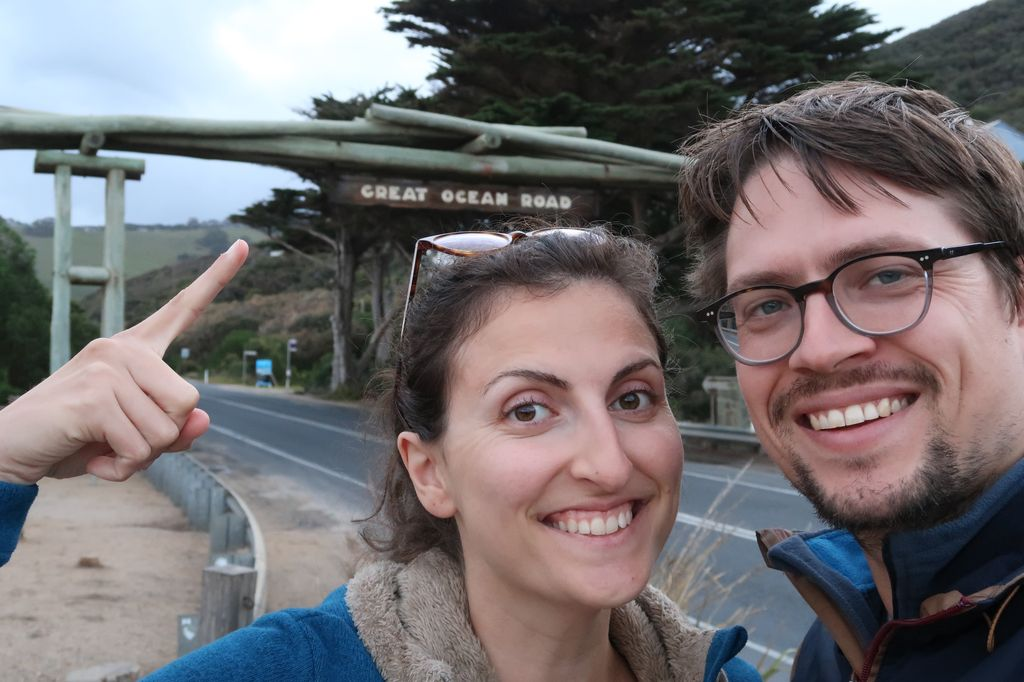
\includegraphics{images/20180731_greatoceanroad.JPG}
\caption{Sous la porte d'entrée de la Great Ocean Road.}
\end{figure}

Certains la visitent en une journée express, nous on avait la chance
d'avoir plein de temps, on l'a donc parcourue en cinq jours qui peuvent
se découper en quatre étapes. Et on en a pris plein les yeux !

\begin{figure}
\centering
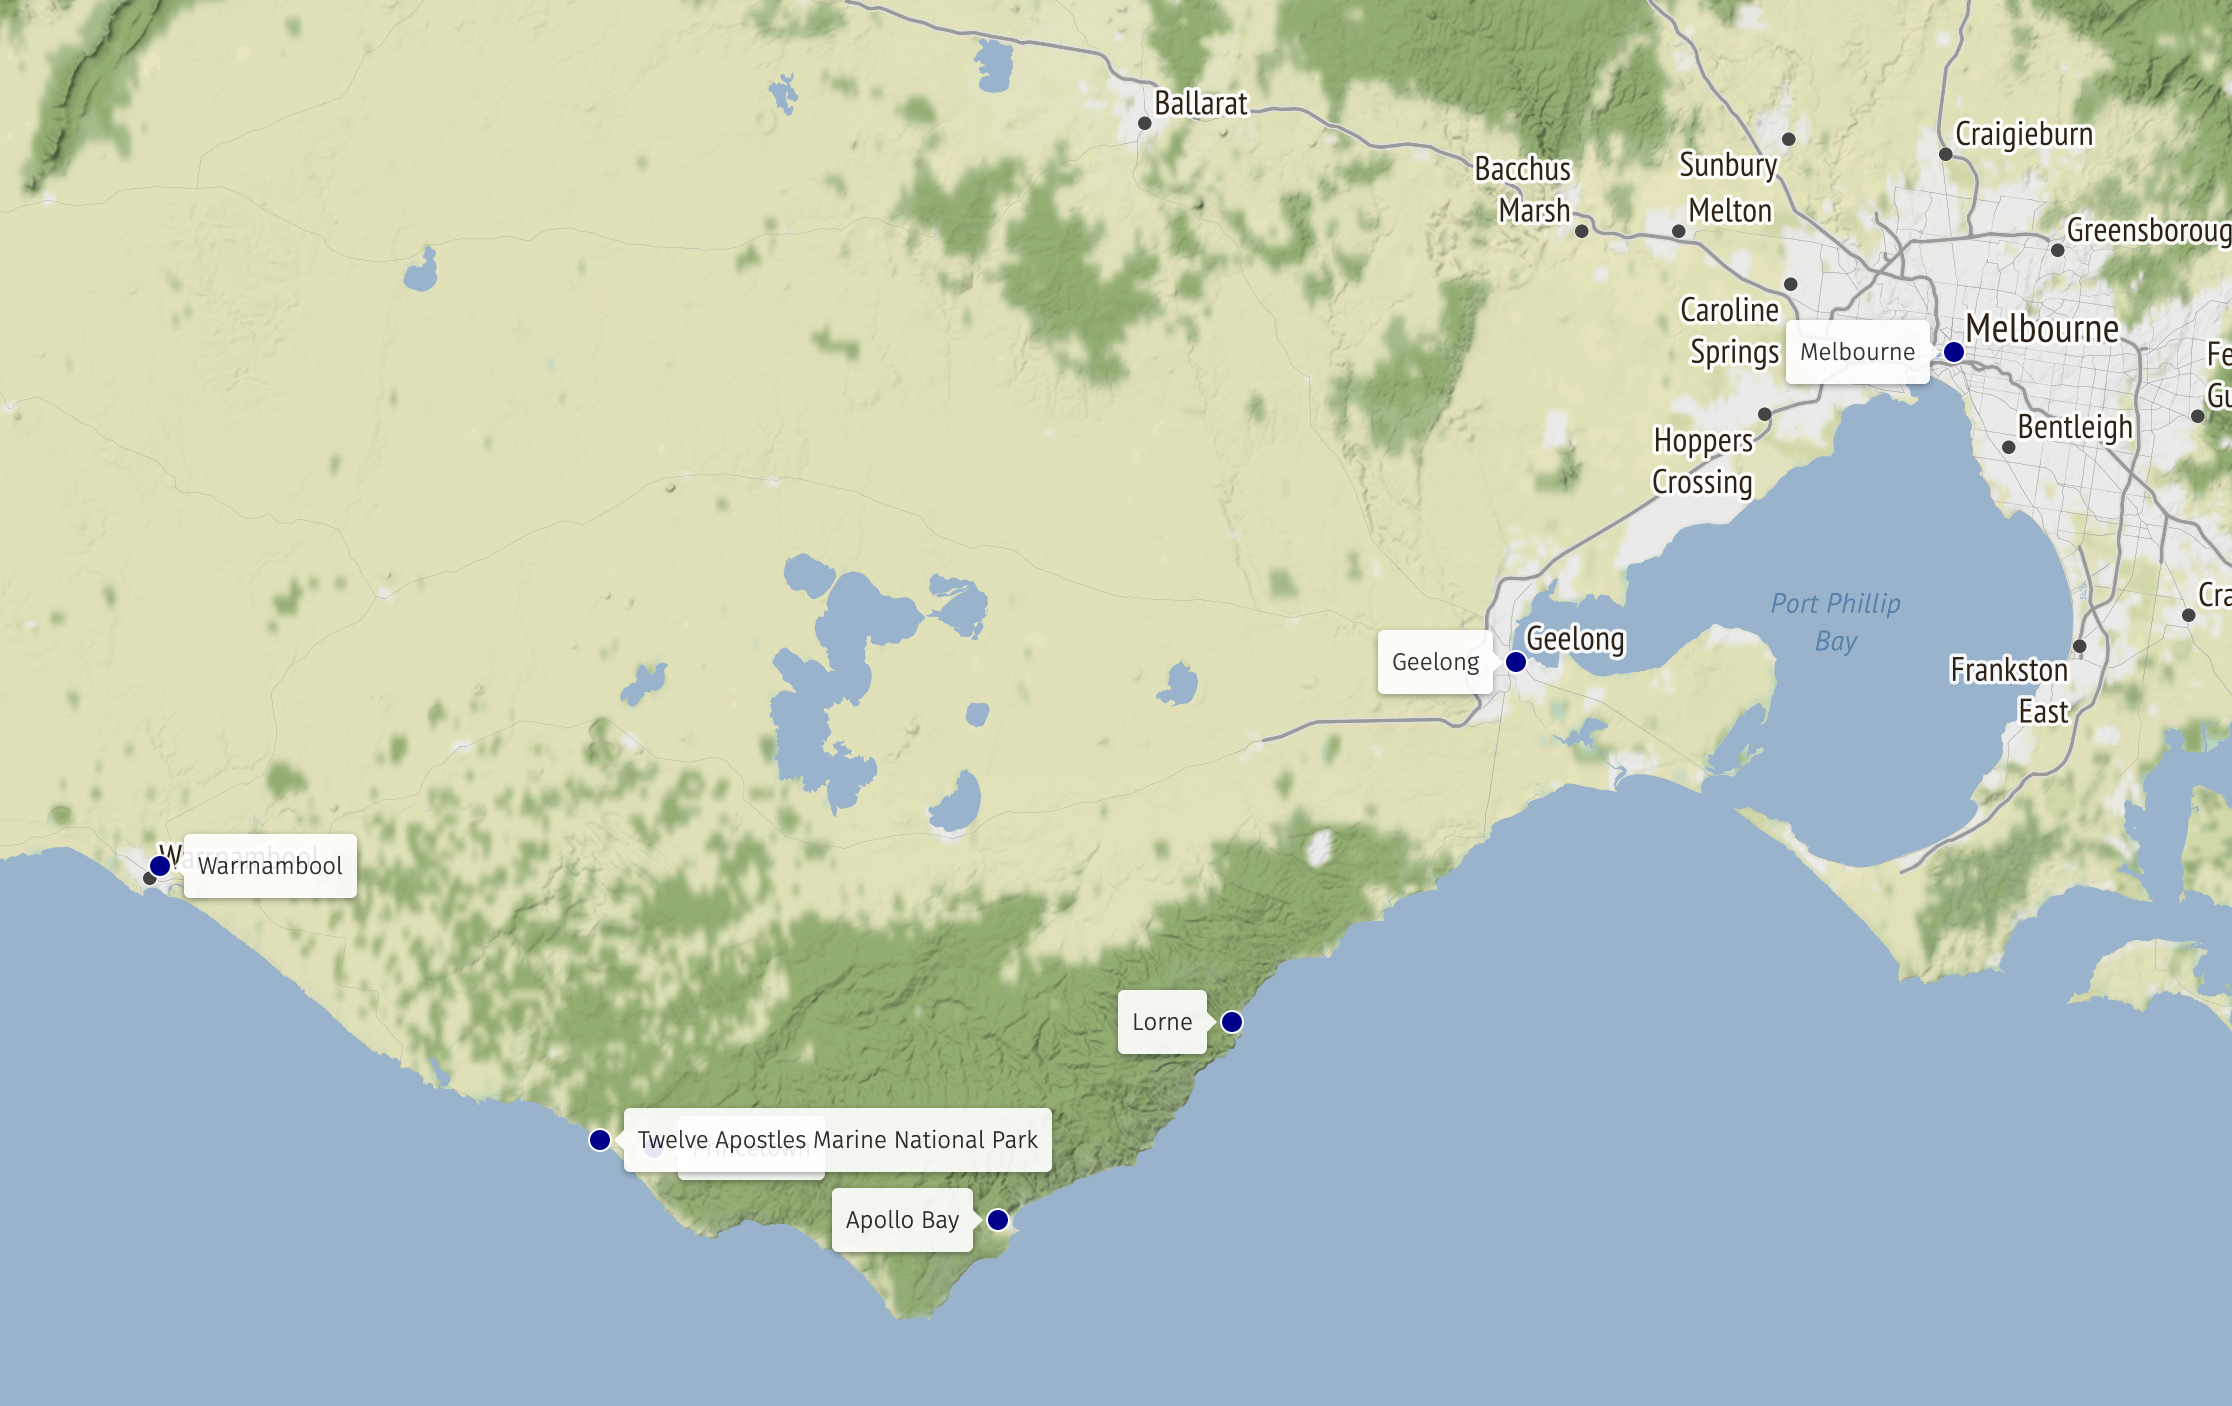
\includegraphics{maps/great_ocean_road.png}
\end{figure}

\hypertarget{de-geelong-uxe0-lorne}{%
\subsection{De Geelong à Lorne}\label{de-geelong-uxe0-lorne}}

La première partie du trajet nous a menés par Geelong que nous n'avons
vue que très rapidement sous une météo capricieuse, puis Torquay et sa
fameuse Bells Beach, siège de compétitions de surf. Nous nous sommes
ensuite arrêtés à Anglesea, où nous avons rencontré pour la première
fois de charmants kangourous, qui vivent leur vie au milieu des
golfeurs. Après un dernier arrêt au phare de Aireys Inlet et ses vues
magnifiques, nous avons fini la journée à Lorne, petite ville
touristique coincée entre la côte et les denses forêts du Otway National
Park. Nous avons gardé une journée entière pour explorer Lorne, où on
trouve de nombreuses occasions d'admirer la nature avoisinante avec pas
moins de dix chutes d'eau accessibles par des sentiers forestiers. On y
a aussi aperçu une baleine depuis le débarcadère !

\begin{figure}
\centering
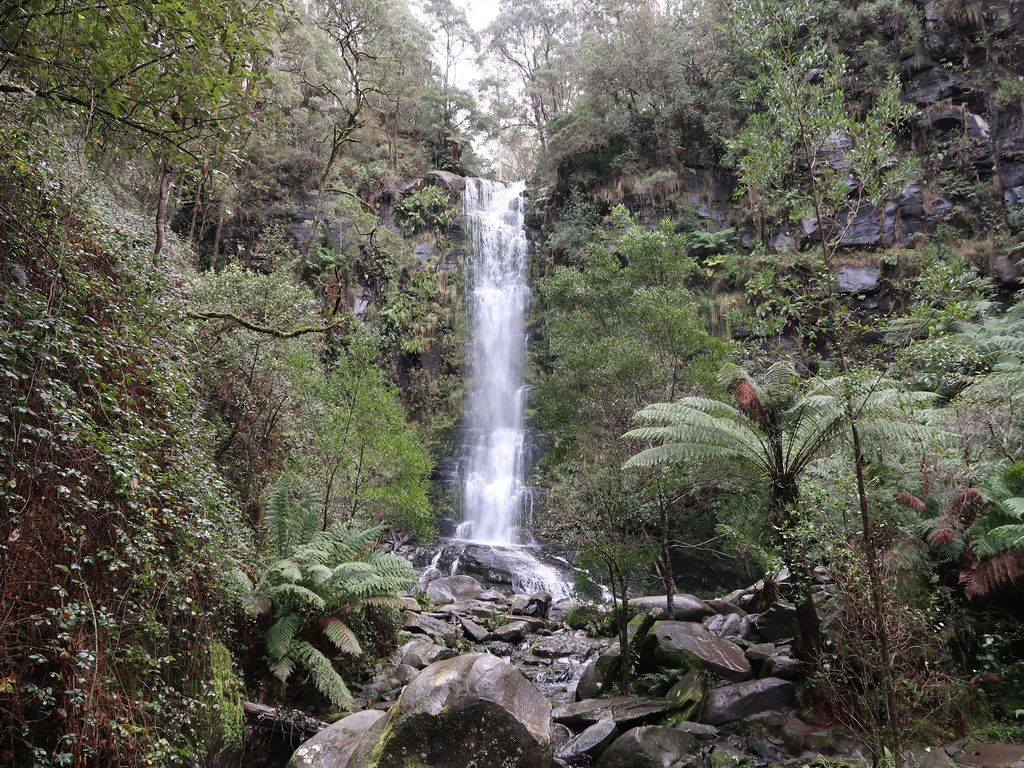
\includegraphics{images/20180731_erskinefalls.JPG}
\caption{Erskine Falls, l'une des cascades recommandées par l'office du
tourisme local.}
\end{figure}

\hypertarget{de-lorne-uxe0-apollo-bay}{%
\subsection{De Lorne à Apollo bay}\label{de-lorne-uxe0-apollo-bay}}

Le moment clé de cette portion de la route aura incontestablement été
l'observation des koalas dans la forêt d'eucalyptus à Kennett River. On
a appris qu'il fallait beaucoup de patience et de concentration pour
repérer ces boules de poils grises qui passent leur temps à dormir en
haut des eucalyptus, mais ça a payé : en remontant la Grey River Road,
nous avons eu la chance d'en compter au moins sept ! Avec en prime
encore et toujours des vues magnifiques sur la forêt et l'océan, une
fois arrivés en haut de la montagne. A Apollo Bay, le Marriner's lookout
nous a offert de magnifiques paysages avec des pâturages d'un côté, et
l'interminable plage de l'autre, de quoi bien finir la journée !

\begin{figure}
\centering
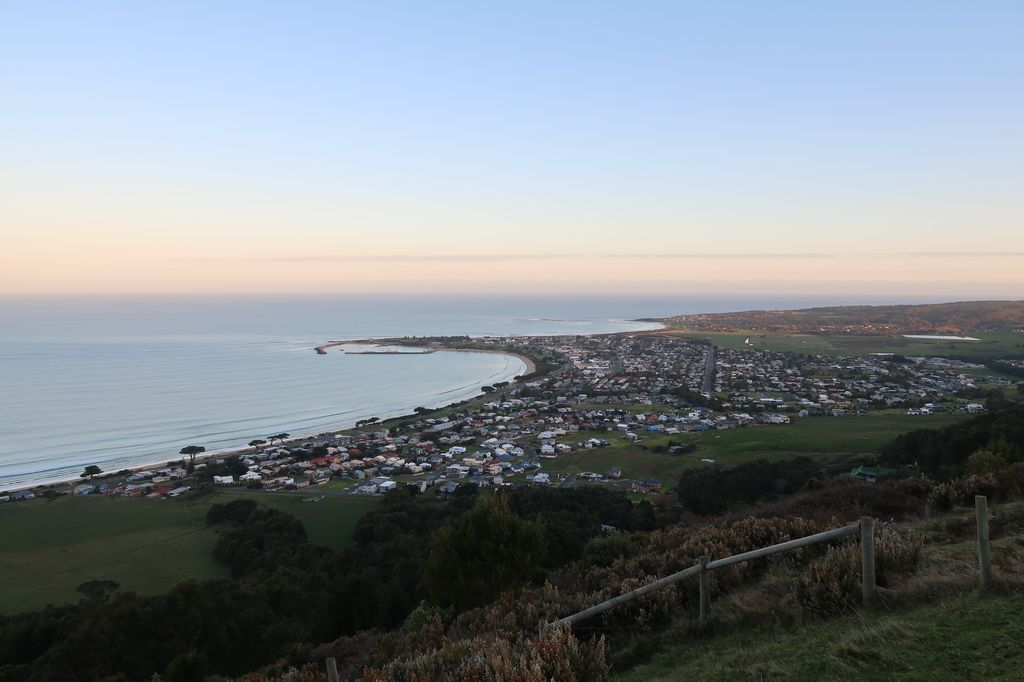
\includegraphics{images/20180731_apollobay.JPG}
\caption{La baie d'Apollon au soleil couchant.}
\end{figure}

\hypertarget{dapollo-bay-jusquuxe0-princetown}{%
\subsection{D'Apollo bay jusqu'à
Princetown}\label{dapollo-bay-jusquuxe0-princetown}}

Après une balade au sanctuaire marin de Marengo Reefs, où nous espérions
croiser la colonie de phoques qui séjourne par là (mais qui ne se sont
pas montrés ce jour-là), l'excursion de la journée nous a amené à Cape
Otway, l'un des premiers phares construits en Australie. L'histoire du
coin est en effet riche en naufrages, de nombreux vaisseaux en
provenance d'Angleterre ayant été victimes des récifs qui s'étendent
jusqu'à 8 km des côtes par endroits. Les guides nous ont également
sensibilisés à la cause aborigène, qui reste aujourd'hui encore un point
de conflit interne en Australie.

\begin{figure}
\centering
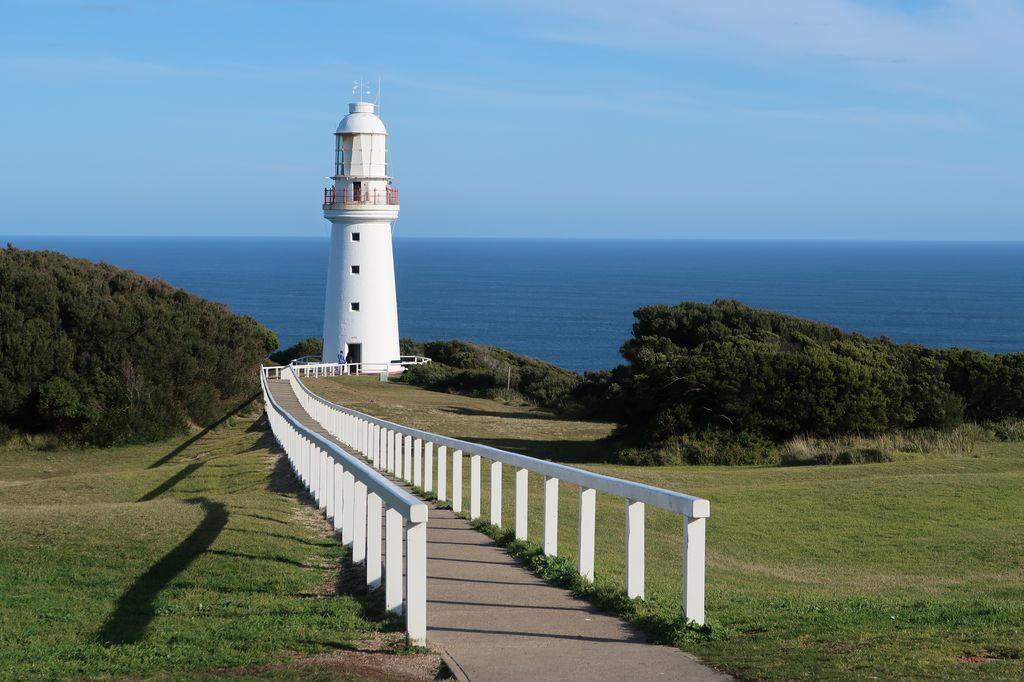
\includegraphics{images/20180731_capeotway.JPG}
\caption{Le phare de Cape Otway.}
\end{figure}

\hypertarget{de-princetown-uxe0-warrnambool}{%
\subsection{De Princetown à
Warrnambool}\label{de-princetown-uxe0-warrnambool}}

Sans aucun doute le segment le plus fréquenté de cette route
touristique. De nombreux arrêts ont été aménagés dû aux belles
formations rocheuses en bordure de côte que l'on y trouve. La plus
célèbre, ce sont les Douze Apôtres, des roches dressées dans la mer qui
les érode peu à peu (et qui sont sept, non-pas douze !). La journée a
été ponctuée par des orages et des averses de grêle, pendant lesquels on
attendait sur le parking la prochaine éclaircie pour nous permettre de
jeter un coup d'œil aux sites... On a donc quand même pu s'arrêter à
Loch Ard Gorge, London Arch, The Grotto, Bay of Islands, pour ne citer
que les principaux. On a globalement fini trempés, mais la lumière au
moment des accalmies était très belle, et on a même gagné quelques
arc-en-ciels en bonus !

\begin{figure}
\centering
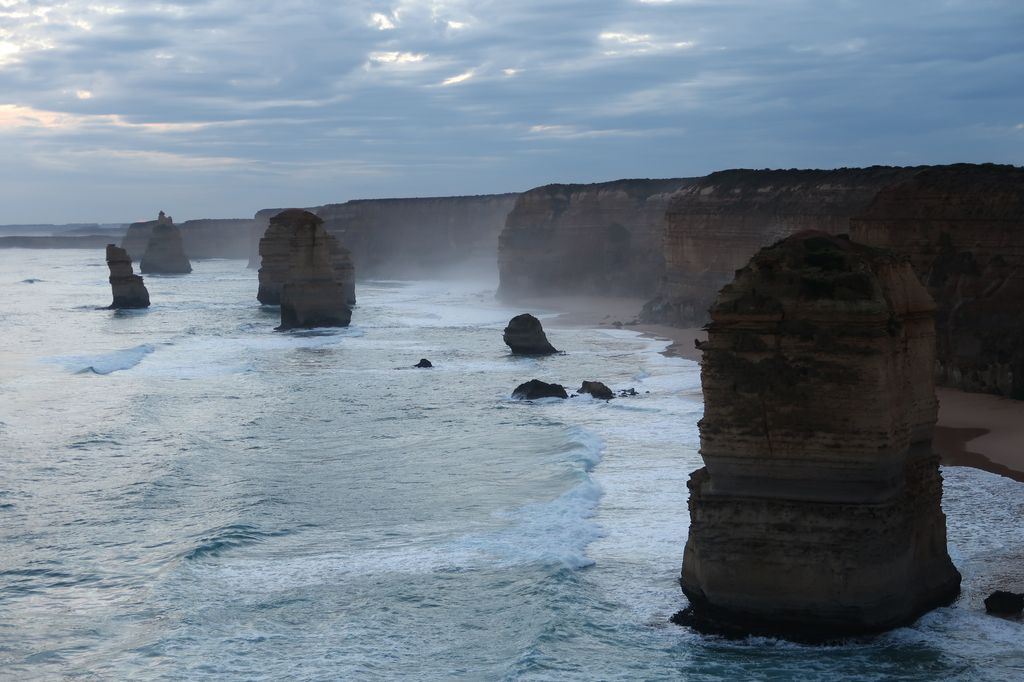
\includegraphics{images/20180731_douzeapotres.JPG}
\caption{Les Douze Apôtres en fin de journée.}
\end{figure}

Après avoir fini de parcourir la Great Ocean Road, nous avons également
fait une brève halte à Melbourne. Nous n'avons pas pu nous y attarder,
mais nous garderons un bon souvenir de la visite guidée de la
bibliothèque d'état du Victoria, dans les tréfonds de laquelle
sommeillent un pendule de Foucault (sans pendule), un ascenseur à
éléphant et des catacombes...

\begin{figure}
\centering
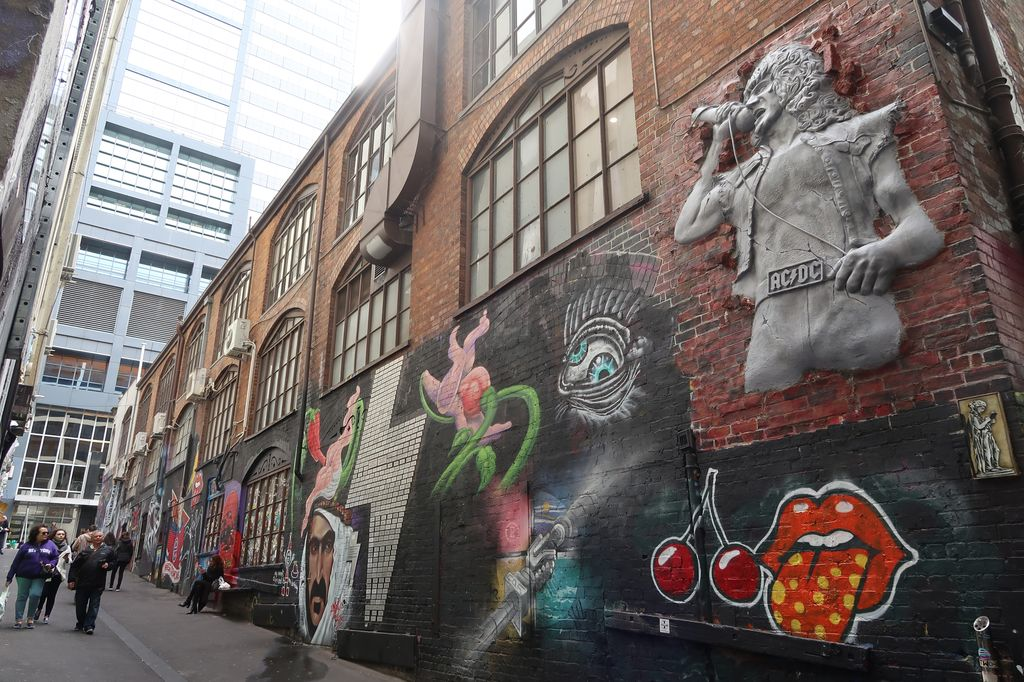
\includegraphics{images/20180731_melbourne.JPG}
\caption{On comprend mieux la solide réputation de ville de street art
qu'a Melbourne quand on arpente ses ruelles.}
\end{figure}

Nous retournons maintenant passer nos dernières journées australiennes à
Sydney, avant de nous envoler pour la Polynésie Française.

\emph{Florian et Elida}
